\section{文本类型数据的输入}

Excel中有三类数据类型
\begin{enumerate}
    \item 数值
    \item 文本
    \item 公式
\end{enumerate}

数值默认右对齐，文本默认左对齐。

\begin{table}[ht]
    \centering
    \begin{tabular}{|c|c|c|}
    \hline
    编号 & 姓名 & 学号 \\ \hline
    01 & 张钧烁 & 2022984150101 \\ \hline
    02 & 张坪 & 2022984150102 \\ \hline
    03 & 展李戎 & 2022984150103 \\ \hline
    04 & 曹骏 & 2022984150104 \\ \hline
    05 & 朱高风 & 2022984150105 \\ \hline
    \end{tabular}
    \end{table}

    \cred{首位是0的数字，0不显示？}

    \cred{位数很多的数字，自动转换成科学计数法？}

    解决办法：
    \begin{enumerate}
        \item 设置单元格格式为文本型
        \item 数字前加单引号
    \end{enumerate}

\section{自动填充}

数值型单元格，拖动默认进行单元格复制；文本型单元格，如果有数字，拖动默认填充序列。

    \begin{minipage}{0.4\linewidth}
        \begin{enumerate}
            \item 通过自动填充选项按钮修改
            \item 按住Ctrl键+鼠标左键下拉，切换模式
            \item 按住鼠标右键下拉，填充序列
            \item 填写多个单元格后，下拉
        \end{enumerate}
    \end{minipage}
    \begin{minipage}{0.4\linewidth} 
        \centering    
        \begin{tabular}{|l|r|}
            \hline
            121 \qquad \quad & \qquad  121 \\ \hline
            122 & 121 \\ \hline
            123 & 121 \\ \hline
            124 & 121 \\ \hline
            125 & 121 \\ \hline
        \end{tabular}            
    \end{minipage}

\cred{office2019及之后版本没有自动填充选项按钮？}

点击“文件”-“选项” -“高级” -“剪贴，复制和粘贴” 下的 “粘贴内容时显示粘贴选项按钮”

点击前面的方框，勾选。

\begin{figure}[ht]
    \centering
    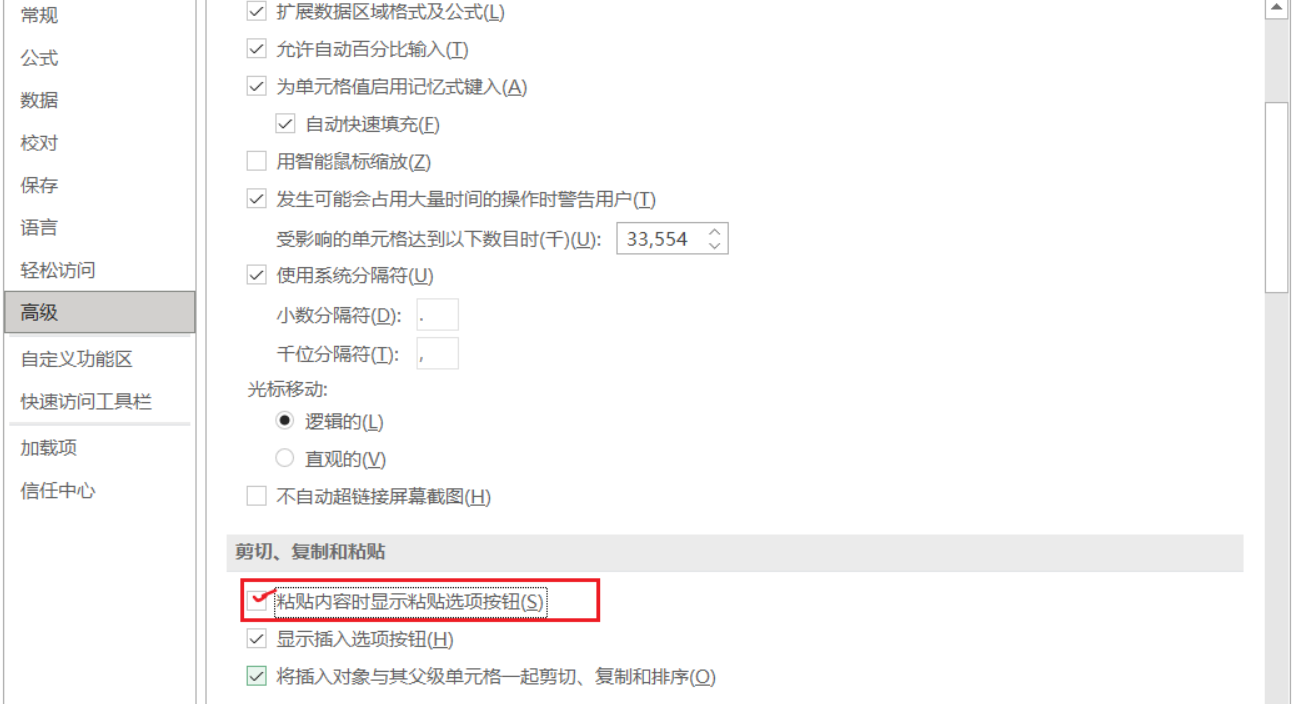
\includegraphics[width=\linewidth]{figures/autofill.png}
\end{figure}

Excel中可自动填充的序列有：
\begin{figure}[ht]
    \centering
    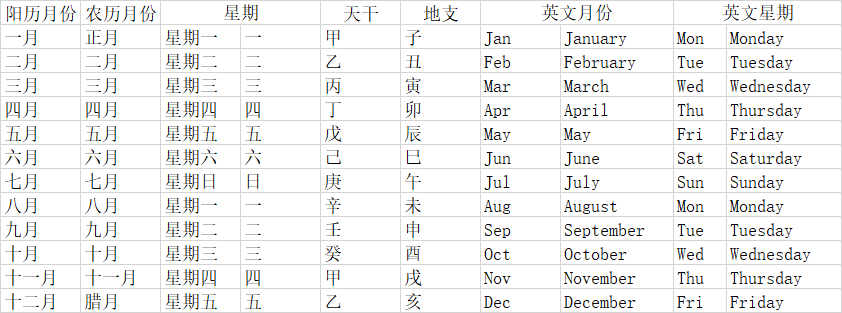
\includegraphics[width=\linewidth]{figures/autofill2.png}
\end{figure}